\documentclass[12pt, a4paper, tocpage=plain]{abnt} % Fonte tamanho 12, papel A4, páginas do sumário sem o p.<número da página>

\usepackage[brazilian]{babel} % Gera datas e nomes em português com estilo brasileiro
\usepackage{hyperref} % Permite a criação de hyperlink no documento, como os links usados na referência
\usepackage[utf8]{inputenc} % Dá suporte para caracteres especiais como acentos e cedilha
\usepackage[T1]{fontenc}
\usepackage[alf]{abntcite} % Define o estilo de referência bibliográfica
\usepackage{graphicx} % Permite a utilização de imagens no documento
\usepackage[small]{caption} % Define as legendas das figuras com fontes menores do que o texto
\usepackage{pslatex} % Define que o formato da letra será Times New Roman
\usepackage{epigraph} % Permite a criação de epígrafes
\usepackage{setspace} % Permite a definição de espaçamento entre linhas
\usepackage[top=3cm, left=3cm, right=2cm, bottom=2cm]{geometry} % Define as margens da folha

\usepackage{listings}
\usepackage{color}
 
\definecolor{dkgreen}{rgb}{0,0.6,0}
\definecolor{gray}{rgb}{0.5,0.5,0.5}
\definecolor{mauve}{rgb}{0.58,0,0.82}
 
\lstset{
  language=Ruby,                % the language of the code
  numbers=left, %numeração de linhas à esquerda
  stepnumber=1,
  firstnumber=1,
  numberstyle=\tiny,
  extendedchars=true,
  frame=none,
  basicstyle=\footnotesize,
  stringstyle=\ttfamily,
  showstringspaces=false,
  captionpos=b,
  %language=Java, %deve ser definida na inclusão de cada trecho de código, pois podem existir linguagens diferentes em exemplos diferentes
  breaklines=true,
  breakautoindent=true,
  %estilos de comentário de uma e várias linhas
  keywordstyle=\color{blue},          % keyword style
  commentstyle=\color{dkgreen},       % comment style
  stringstyle=\color{mauve},         % string literal style
  frame=single,                   % adds a frame around the code
  extendedchars=\true,
  inputencoding=utf8,
}

\setcounter{secnumdepth}{3} % Até três subsubsections numeradas
\setcounter{tocdepth}{3} % Até trẽs subsubsections numeradas

\setlength{\parindent}{1.25cm} % Define o recuo da primeira linha dos parágrafos para 1.25 cm

\renewcommand{\ABNTchapterfont}{\bfseries} % Define a fonte do \chapter
\renewcommand{\ABNTchaptersize}{\large} % Define o tamanho da fonte do \chapter
\renewcommand{\ABNTsectionfontsize}{\large} % Define o tamanho da fonte da \section
\renewcommand{\ABNTsubsectionfontsize}{\large} % Define o tamanho da fonte do \subsection
\renewcommand{\ABNTsubsubsectionfontsize}{\large} % Define o tamanho da fonte do \subsubsection
\renewcommand{\ABNTbibliographyname}{REFERÊNCIAS BIBLIOGRÁFICAS} % Modifica o título gerado pelo \bibliographys

\renewcommand{\lstlistingname}{Código} % Codigo

\begin{document} % Começo do TCC
\begin{titlepage}
 \begin{figure}[ht]
 \centering
 \scalebox{0.55}{
\includegraphics{figuras/logo}}
 \end{figure}
 \begin{center}
   {\large BACHAREL EM SISTEMAS DE INFORMAÇÃO} \\ [3.5cm]
   {\large TIAGO SAMAHÁ CORDEIRO} \\ [4cm]
   {\large DOCUMENTAÇÃO EXECUTÁVEL} \\ [0.5cm]
   {\small UM ESTUDO DE CASO DA BIBLIOTECA DIGITAL DA EPCT} \\
   \vfill
   {\large Campos dos Goytacazes/RJ} \\
   {\large 2012}
 \end{center}
\end{titlepage} % Cria a capa
\begin{titlepage}
 \begin{figure}[ht]
 \centering
 \scalebox{0.55}{
\includegraphics{figuras/logo}}
 \end{figure}
 \begin{center}
   {\large BACHAREL EM SISTEMAS DE INFORMAÇÃO} \\ [3.5cm]
   {\large TIAGO SAMAHÁ CORDEIRO} \\
   {\large NATANAEL DE ARAÚJO SILVA} \\ [4cm]
   {\large NSI-BD-TOUR}\\ [0.5cm]
   {\small DOCUMENTAÇÃO EXECUTÁVEL NA BIBLIOTECA DIGITAL DA EPCT} \\ [2.5cm]
   \hspace{.45\textwidth} % posicionando a minipage
   \begin{minipage}{0.53\textwidth}
   \begin{espacosimples}
      Trabalho de conclusão de curso apresentado ao Instituto Federal Fluminense como requisito parcial para conclusão do Bacharel em Sistemas de Informação.\\[1.5cm]
      Orientador: Prof. Rogério Atem de Carvalho, DSc
      Co-orientador: Prof. Fernando Luiz de Carvalho e Silva, MSc
    \end{espacosimples}
    \end{minipage}
   \vfill
   {\large Campos dos Goytacazes/RJ} \\
   {\large 2012}
 \end{center}
\end{titlepage} % Cria a folha de rosto
\begin{folhadeaprovacao}
    \setlength{\ABNTsignthickness}{0.4pt}
    \setlength{\ABNTsignwidth}{15cm}
    \setlength{\ABNTsignskip}{0.9cm}
    \begin{center}
        {\large TIAGO SAMAHÁ CORDEIRO*} \\
        {\large NATANAEL DE ARAÚJO SILVA**} \\ [1cm]
        {\large DOCUMENTAÇÃO EXECUTÁVEL}\\ [0.5cm]
		{\small UM ESTUDO DE CASO NA BIBLIOTECA DIGITAL DA EPCT} \\ [1cm]
        \hspace{.47\textwidth} % posicionando a minipage
        \begin{minipage}{0.5\textwidth}
        \begin{espacosimples}
        Trabalho de conclusão de curso apresentado ao Instituto Federal Fluminense como requisito parcial para conclusão do Bacharel em Sistemas (*) de Informação e Tecnólogo em Desenvolvimento de Software (**).\\\\
        \end{espacosimples}
        \end{minipage}
    \end{center}
    Aprovada em 19 de julho de 2012 \\\\
    Banca avaliadora:
    \assinatura{Prof. Rogério Atem de Carvalho, DSc (Orientador) \\ Doutor em Engenharia de Produção \\ Instituto Federal Fluminense / Campus Campos Centro}
    \assinatura{Prof. Fernando Luiz de Carvalho e Silva, MSc (Co-Orientador) \\ Mestre em Engenharia de Produção \\ Instituto Federal Fluminense / Campus Campos Centro}
    \assinatura{Prof. Luiz Gustavo Lourenço Moura, DSc \\ Doutor em Computação \\ Instituto Federal Fluminense / Campus Campos Centro}
        \assinatura{Prof. Vinícius Barcelos da Silva, MSc \\ Mestre em Engenharia de Produção \\ Instituto Federal Fluminense / Campus Campos Centro}
\end{folhadeaprovacao} % Cria a folha de aprovação
\null
\vfill

{\normalsize \it \hfill Aos nossos pais.}  % Cria a folha de dedicatória
\begin{center}
\textbf{AGRADECIMENTOS}
\end{center}

Quero agradecer a Deus, pois sem ele nada seria possível, minha família que me apoiou em todas decisões, meus colegas de trabalho que sempre ajudaram-me e ao NSI/IFF por me proporcionar recursos financeiros e materiais para o desenvolvimento deste trabalho.

Tiago Samaha

Primeiramente agradeço a Deus, pois sem Ele nada seria possível. Agradeço aos meus pais, Nilton e Eliana, pelo imenso amor e dedicação que sempre recebi e por acreditarem e investirem em mim. À minha namorada e companheira Bia, lua da minha vida, que sempre me escuta, ajuda e incentiva. Aos meus queridos amigos pelo companheirismo e pelas palavras amigas.

Agradeço aos excelentes professores com quem tive a oportunidade e o prazer de aprender, são vocês os culpados pela minha paixão por computação. Ao NSI/IFF e aos amigos que lá fiz. Em especial agradeço ao professor Fernando, que sempre esteve presente, auxiliando, orientando e incentivando, sem ele certamente esse trabalho não seria possível.

Natanael de Araújo Silva % Cria a folha de agradecimentos
\null % o \vfill só funciona com o \null
\vfill
\epigraph{Estou do lado de Aslam, mesmo que não haja Aslam. Quero viver como um narniano, mesmo que Nárnia não exista.}{Brejeiro}
 % Cria a epígrafe (onde se coloca um pensamento)
\begin{center}
\textbf{RESUMO}
\end{center}
\singlespacing

\noindent O objetivo deste trabalho é apresentar o conceito de documentação executável, aplicada no projeto da Biblioteca Digital como uma evolução da documentação tradicional, trazendo como vantagens adicionais a possibilidade do treinamento dos usuários e a validação das funcionalidades pelo cliente. Além disso, este formato de documentação também tende a manter-se atualizado mais facilmente, já que além de documentar, a mesma assume outras funcionalidades, agregando mais valor ao usuário. Assim, como resultados diretos, este trabalho contribui com o projeto da Biblioteca Digital da SETEC/EPCT, criando um módulo de documentação executável e descreve o emprego das bibliotecas \textit{Amberjack2} e jQuery na implementação de documentação executável. \\

\noindent PALAVRAS-CHAVE: documentação executável, testes automatizados, treinamento
 % Resumo do trabalho
\begin{center}
\textbf{ABSTRACT}
\end{center}
\singlespacing

\noindent The aim of this work is to present the concept of Executable Documentation as an evolution of traditional documentation, which brings advantages such as the possibility of user training and requirements validation. Additionally, this format of documentation tends to keep synchronized with the source code, while documenting, training takes place, adding more value to the user. Therefore, a case study was implemented on the EPCT Digital Library, having as a direct result the creation of an executable documentation module for that application, as well as the description of the use of Amberjack2 and jQuery libraries to implement executable documentation. \\


\noindent KEYWORDS: executable documentation, automated tests, training % Resumo em língua estrangeira
\renewcommand{\listfigurename}{LISTA DE FIGURAS} % Modifica o nome da lista de figuras
\listoffigures % Gera o índice de figuras
\renewcommand{\listtablename}{LISTA DE TABELAS}
\listoftables % Gera o índice de tabelas
\renewcommand{\lstlistlistingname}{LISTA DE CÓDIGOS}
\lstlistoflistings
\renewcommand{\contentsname}{SUMÁRIO} % Modifica o nome do sumário
\tableofcontents % Gera o sumário
\onehalfspacing % Define o espaçamento de 1.5cm entre linhas
\chapter{INTRODUÇÃO}

Para lidar com a dinâmica da economia atual, empresas de software estão sofrendo fortes pressões para desenvolver sistemas de informação em prazos cada vez menores, uma vez que existem muitos clientes não satisfeitos com a qualidade eu tempo de entrega dos sistemas. Tais sistemas precisam ser escaláveis e integrados com outros sistemas existentes ou em desenvolvimento. Os ambientes tecnológicos nos quais estes sistemas são desenvolvidos estão em constante evolução devido a solicitações do cliente \cite{CRESPO}.

As metodologias tradicionais de desenvolvimento de software já não se adequam às demandas atuais por agilidade na mudança e flexibilidade na sua construção, em especial no caso dos softwares voltados para gestão organizacional. Em um projeto tradicional, os programadores recebem uma documentação inicial, que descreve o que o software deve fazer, e precisam transformar o texto escrito em código.

Com as constantes modificações dos requisitos do sistema que visam acompanhar os processo de negócio, a sincronização da documentação torna-se um grave problema. Documentos escritos em papel, ou até mesmo digitalizados, precisam de pessoas para mantê-los atualizados e estão mais sujeitos a erros, por faltar sincronia com o código fonte, que, em última instância, é o que realmente faz o software funcionar. Pior que ter documentação em excesso é ter documentação errada. É preferível ter pouca documentação a ter uma grande quantidade de documentação com erros, pois estes podem levar a mal-entendidos que resultarão em prejuízos - tais como dias de trabalho perdido \cite{NSI}.

Um outro grande problema no processo de desenvolvimento de software é conseguir garantir que todos os requisitos solicitados pelo cliente realmente estão funcionando como esperado, assim surge a necessidade de criar testes automatizados que cubram todos os requisitos solicitados. Testes automatizados são programas ou scripts simples que monitoram funcionalidades do sistema sendo testado e fazem verificações automáticas nos resultados obtidos. A grande vantagem desta abordagem, é que todos os casos de teste podem ser facilmente e rapidamente repetidos a qualquer momento e com pouco esforço. Além disso, testes automatizados são uma boa documentação para o desenvolvedor \cite{KON}.

A solução destes problemas é a utilização de testes automatizados – código que verifica código – associados a chamada documentação executável. Entende-se por documentação executável, a definição de cenários expressos de execução do sistema de informação pelo cliente em linguagem natural, que permitem definição e manutenção de requisitos que irão validar e verificar o software desenvolvido. Assim o cliente terá uma documentação que irá garantir a qualidade do software, além de ajudar no treinamento de utilização do mesmo.

\section{Justificativa do trabalho}

Através deste trabalho desejamos criar um material que se torne referência, uma vez que não se encontra na literatura amplo material sobre o assunto. O desenvolvimento de uma ferramenta de documentação executável foi o tema escolhido para este trabalho através do contato de um parceiro industrial (Nexedi SA) do Núcleo de Pesquisa em Sistemas de Informação (NSI), que desenvolve pesquisas em sistemas integrados de gestão.

\section{Objetivo}

O objetivo deste projeto é integrar a aplicações web (portais, sistemas integrados de gestão), uma ferramenta que permite ao usuário final executar cenários – tutorial guiado – objetivando a validação dos requisitos do sistema. Desta forma, é possível simultaneamente validar os requisitos do sistema e guiar o usuário no emprego do sistema. % Cria o capítulo 1
\chapter{FUNDAMENTAÇÃO TEÓRICA}

Neste capítulo e apresentada uma revisão de assuntos relacionados na literatura, visando embasamento conceitual, para o entendimento deste trabalho.

\section{Origem dos testes na indústria}

Desde do início da indústria percebeu-se que os produtos precisam estar adequados a especificação. Produtos que são terminados com inconformidades tornam a produção mais lenta, gerando desperdícios como adaptação, retrabalho e refugo. O mesmo ocorre no processo de desenvolvimento de software, onde cada requisito deve atender as especificações solicitadas pelo cliente, caso contrário poderá ter funcionalidades inadequadas ou desnecessárias, que levam aos mesmos problemas da indústria.

A solução utilizada no secúlo XX, foi a inspeção ao final da produção. A indústria ocidental evoluiu ao fazer inspeções proativas (no estoque) e estatísticas por período de tempo. Entretanto o tempo entre a geração do erro e sua identificação diminui a capacidade de identificação da causa raíz dos problemas e de sua solução \cite{CARVALHO}.

Segundo \citeonline{HOLWEG}, em 1918 Sakichi Toyoda implantou em sua indústria de tecelagem uma máquina que verifica a linha de produção. Ao detectar anormalidades, como por exemplo a falta ou quebra da linha, a produção era parada e os operadores avisados, evitando assim a necessidade de operários para monitoramento da produção, e que o produto não atendesse a especificação. Desta maneira o tempo de identifição do problema é curto, evita vários problemas no processo de produção e aumenta as chances de análise e identificação das causas dos problemas.

Entretanto, todo o conhecimento gerado na industria oriental passou desapercebido, sem publicações científicas, até a década de 90, quando se iniciaram pesquisas a este respeito. Sendo assim, até os dias de hoje, percebe-se grandes falhas em empreendimentos nas diversas formas de indústria, inclusive na indústria de software.

\section{Prejuízos na indústria de software}

Software são desenvolvidos a mais de cinquenta anos e ainda tem grandes problemas com a qualidade e garantia de entrega. Segundo \citeonline{CHARETTE}, bilhões de dólares são gastos em projetos  que não são terminados, e 5\% a 15\% dos projetos iniciados serão abandonados antes de serem entregues ou considerados totalmente inadequados logo depois de seu término.

Desenvolver sistemas é caro, e o processo frequentemente sofre dificuldades com as metodologias adotadas, muitas delas não se adequam as atuais exigências do mercado. Por exemplo, o gerente do projeto e os desenvolvedores, devem estar sempre preparados para avaliar as demandas passadas pelos seus clientes (stakeholders) durante o processo de desenvolvimento do sistema. Na etapa de codificação, surgem constantes solicitações de modificações dos requisitos, os quais podem afetar o custo e a qualidade do software \cite{CERPA}.

O maior problema no processo de desenvolvimento é a existência de falhas no sistema, principalmente as detectáveis e previsíveis. Porém, muitas organizações ainda não consideram que a prevenção e detecção de falhas através de testes seja importante, mesmo que possam correr o risco de causar prejuízos ao cliente \cite{CHARETTE}. A tabela \ref{falhas_em_projetos} exemplifica tipos de falha em projetos de desenvolvimento de software é apresentada abaixo.

\begin{table}[ht]
	\centering
	\fontsize{8}{0}
	\caption{Percentual de projetos falhos por fator de falha}
	\label{falhas_em_projetos}
\begin{tabular}{lccc}

\hline

\textbf{Fatores de falha em projetos de software} & \multicolumn{3}{c}{\textbf{Porcentagem de projetos (\%)}}\tabularnewline

\cline{2-4}

& \textbf{In-House} & \textbf{Outsourced} & \textbf{Geral}\tabularnewline

\hline

Data de entrega influenciou no processo & 93,9 & 90,5 & 92,9\tabularnewline

\hline

Projeto estimado por baixo & 83,7 & 76,2 & 81,4\tabularnewline

\hline

Riscos não fora reavaliados, controlados ou gerenciados & 73,4 & 80,9 & 75,7\tabularnewline

\hline

A gerência não foi recompensada por longas horas de trabalho & 81,6 & 57,1 & 74,3\tabularnewline

\hline

Tomada de decisão foi feita sem informações necessárias & 83,7 & 47,6 & 72,9\tabularnewline

\hline

A gerência teve experiência desconfortável & 83,7 & 47,6 & 72,9\tabularnewline

\hline

Clientes não envolvidos na preparação do cronograma & 69,4 & 76,2 & 71,4\tabularnewline

\hline

Risco não está incorporado no planejamento do projeto & 65,3 & 80,9 & 70,0\tabularnewline

\hline

Controle de mudanças não monitorado/negociado efetivamente & 63,3 & 85,7 & 70,0\tabularnewline

\hline

Clientes e usuários tiveram espectativas não realísticas & 69,4 & 66,7 & 68,6\tabularnewline

\hline

Processo não teve revisões ao final de cada fase & 75,5 & 47,6 & 67,1\tabularnewline

\hline

Metodologia não apropriada para o projeto & 71,4 & 52,4 & 65,7\tabularnewline

\hline

Cronograma agressivo afetou a motivação da equipe & 69,4 & 57,1 & 65,7\tabularnewline

\hline

Mudanças no escopo durante o projeto & 67,3 & 57,1 & 64,3\tabularnewline

\hline

Cronograma teve efeito negativo na vida dos elementos da equipe & 71,4 & 42,9 & 62,9\tabularnewline

\hline

Projeto com equipe inadequada para cumprir o cronograma & 63,3 & 57,1 & 61,4\tabularnewline

\hline

Equipe adicionada tardiamente para cumprir um cronograma & 61,2 & 61,9 & 61,4\tabularnewline

\hline

Clientes não dão tempo suficiente para levantar requisitos & 61,2 & 57,1 & 60,0\tabularnewline

\hline

\end{tabular}
\end{table}

\section{Filosofia de Teste de Software}

Teste de software é uma das mais importantes atividades na garantia de qualidade. Segundo \citeonline{PRESSMAN}, a atividade de teste em um projeto de software pode consumir 40\% do esforço total do mesmo e chegar a custar de três a cinco vezes mais que todas as outras etapas da engenharia de software somadas.

A definição comumente aceita da atividade de teste de software é a de que "teste de software consiste de uma série de procedimentos pré-definidos para garantir que o código faça o que ele foi projetado para fazer e não tenha nenhum comportamento não desejado". Porém, \citeonline{MYERS}, aponta para o fato de que o objetivo primário de um teste de software é encontrar erros no código e não provar que o programa atinge aos objetivos: "Teste de software é o processo de se executar um programa com o propósito de descobrir erros". 

Muitos programadores assumem uma definição menos eficiente sobre a atividade de teste:

\begin{itemize}
\item A atividade de teste é o processo de demonstrar a inexistência de erros no software
\end{itemize}

Esse pensamento comum é inapropriado pois apesar da atividade de teste poder descobrir defeitos no software, ela é incapaz de mostrar a inexistência destes. No mundo real, é impraticável criar casos de teste para todas as combinações e cenários possíveis para aplicações mais complexas.

\begin{itemize}
\item O propósito da atividade de teste é mostrar que um programa executa suas funções corretamente.
\end{itemize}

Esta definição pode ser considerada incompleta pois mesmo que um programa atinja os objetivos para o qual foi projetado, ainda pode conter erros caso apresente funcionalidades adicionais.

\begin{itemize}
\item Teste de software é o processo de garantir que um programa faz o que foi projetado para fazer.
\end{itemize}

Apesar de uma atividade de teste bem executada poder demonstrar a conformidade entre os requisitos do cliente e as funcionalidades implementadas no software, este é um benefício secundário. Como qualquer outra atividade no processo de desenvolvimento, testes também devem agregar valor ao software, e portanto é importante encontrar defeitos. Neste sentido, a qualidade da atividade de teste será diretamente proporcial ao esforço em encontrar defeitos.

Por tudo isso, percebe-se que os testes de software cumprem uma função ética no processo de desenvolvimento, evitando prejuízos para as organizações ou pessoas. Um exemplo claro disso, é a responsabilidade atribuída ao desenvolvedor do algoritmo presente em um marca-passo, onde qualquer falha pode causar graves prejuízos ao usuário.

Portanto, para conduzir os testes efetivamente, existe toda uma complexidade advinda da variedade de algorítmos que precisarão ser testados. Várias técnicas propostas para endereçar os testes de algorítmos são apresentadas nos tópico a seguir. % Cria o capítulo 2
\chapter{ESTUDO DE CASO}
Este capítulo apresenta um estudo de caso da implementação de uma ferramenta de documentação executável no projeto da Biblioteca Digital.

O estudo de caso foi idealizado devido a necessidade de existir uma documentação que agregue mais valor ao cliente. Documentação executável pode validar requisitos e guiar o usuário no emprego do sistema.

\section{Projeto da Biblioteca Digital} 	 	

A Biblioteca Digital (BD) é um projeto de pesquisa e desenvolvimento que inciou-se em março de 2007, através de uma solicitação da SETEC/MEC ao Núcleo de Pesquisa de Sistemas de Informação (NSI) do Instituto Federal Fluminense. O NSI foi criado em abril de 2002 e desde essa época vem estimulando o uso tecnologias livres para pesquisa e desenvolvimento de software.

O projeto da BD visa disponibilizar um acervo de documentos produzidos pela rede de Instituições de Educação Profissional Científica e Tecnológica (EPCT) – como artigos, monografias, dissertações, teses e periódicos – promovendo a disseminação de conhecimento através destes conteúdos.

Como em todo projeto de desenvolvimento de software, a documentação do sistema é um problema constante. Sincronizar documentos escritos em papel com o código do sistema, é uma tarefa difícil e sujeita a falhas. 

\section{Proposta da ferramenta}

Devido a este problema, foi levantada a necessidade de desenvolver uma ferramenta de documentação executável que permita ao usuário validar requisitos do sistema e guiá-lo na utilização do mesmo. Portanto esta ferramenta tem como objetivos suportar sua documentação e treinar o usuário no emprego do sistema.

Assim, pode-se destacar como vantagens da implantação a otimização do uso do sistema, pois através dos passos estabelecidos o usuário poderá avaliar a simplicidade da execução das ações ou estabelecer outros comportamentos melhorados.

Outra vantagem esperada é a validação dos cenários, onde todos os passos executados foram pré-definidos pela especificação do cliente. Desta maneira pode-se validar interativamente todos os cenários descritos.

A partir da utilização da documentação interativa, os usuários poderão ser facilmente treinados nas funcionalidades da Biblioteca Digital, sem a necessidade de uma tutoria dedicada.

\section{Desenvolvimento}

Neste tópico serão demonstrados os passos executados para realização deste trabalho, possibilitando ao leitor avaliar ou reproduzir os efeitos aqui descritos.

\subsection{Ambiente de desenvolvimento}

O projeto da BD é desenvolvido na linguagem \textit{Ruby} utilizando o \textit{framework} \textit{web Ruby on Rails} \cite{RAILS}. Uma das vantagens de utilizar este \textit{framework} é a existência de um conjunto de bibliotecas que facilitam o desenvolvimento guiado a testes \cite{BECK}.

Durante o processo de desenvolvimento da ferramenta foi utilizada a biblioteca de testes automatizados RSpec \cite{CHELIMSKY}, a qual fornece ao desenvolvedor uma \textit{domain specific language} (DSL), que facilita especificação dos comportamentos esperados do objeto (Código \ref{lst:codigo31}).

{\singlespace
\begin{lstlisting}[caption=Exemplo da DSL do Rspec,label={lst:codigo31}]
describe Person do
  subject {
    Person.new(:name => "John Doe", :role => "moderator")
    }

  its(:name) { should == "John Doe" }

  it "is a admin" do
    subject.role = "admin"
    subject.should be_admin
  end

  it "is not a admin" do
    subject.role = nil
    subject.should_not be_admin
  end

  it "instantiates without hash" do
    expect { Person.new }.to_not raise_error(ArgumentError)
  end
end
\end{lstlisting}
}

O resultado de execução do código acima pode ser visto na Figura \ref{figura_31}, a qual descreve os testes que passaram.

\begin{figure}[ht]
    \centering
    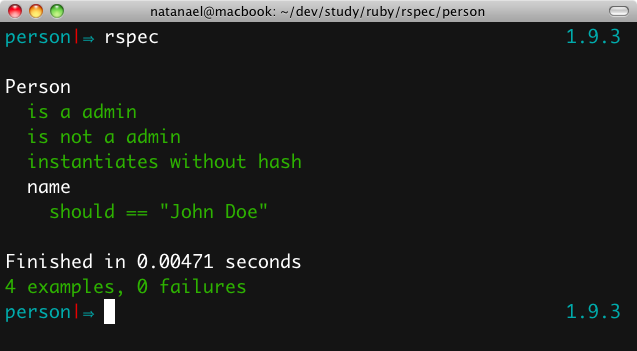
\includegraphics[width=0.9 \textwidth]{figuras/figura_31}
    \caption{Saída após rodar os testes com RSpec}
    \label{figura_31}
\end{figure}

Além da utilização desta biblioteca de testes, foi utilizado o conceito de "passos de bebê", ou seja, pequenas partes são desenvolvidas a cada momento, seja levantamento de requisitos, implementação de funcionalidade, refatoração ou até especificações. Um exemplo disto é focar no desenvolvimento de uma pequena parte de uma funcionalidade, diminuindo o risco do desenvolvimento e asegurando o atingimento de objetivos alcançaveis \cite{RODRIGO}.

\subsection{Testes desenvolvidos}

Todo processo de desenvolvimento da ferramenta utilizou TDD, onde foram criadas verificações unitárias dos \textit{models}, \textit{views} e \textit{controllers}.

Os testes de \textit{model} têm a responsabilidade de especificar e verificar a lógica de negócio da aplicação, avaliando o comportamento dos objetos. O Código \ref{lst:codigo33} mostra o teste responsável pelo \textit{model} \textit{Scenario}.

{\singlespace
\begin{lstlisting}[caption=Teste unitário de \textit{model},label={lst:codigo33}]
describe Scenario do
  it { should_not have_valid(:yaml).when('', nil) }
  its(:yaml) { should be_accessible }

  context "when a yaml file" do
    context "is not given" do
      its(:name) { should eq('') }
      its(:to_param) { should eq("") }
      its(:contexts) { should eq([]) }
      its(:to_hash) { should be_empty }
      its(:to_hash) { should be_a(Hashr) }
    end

    context "is given" do
      subject { Scenario.new yaml: File.read("./spec/resources/scenario.yml") }

      it "#to_hash should return @yaml Hashr" do
        subject.yaml = "hero: _why"
        subject.to_hash.should eq({:hero => '_why'})
        subject.to_hash.should be_a(Hashr)
      end

      it "#url should return the first context url" do
        subject.stub(id: 1)
        subject.url.should eq("/?tourId=1-criar-usuario")
      end
    end
  end
end
\end{lstlisting}
}

A cobertura de testes atumatizados das \textit{views} foram desenvolvidas para verificar se o conteúdo é corretamente apresentado ao usuário na página (Código \ref{lst:codigo34}).

{\singlespace
\begin{lstlisting}[caption=Teste unitário de \textit{view},label={lst:codigo34}]
describe "scenarios/_context.html.erb" do
  before do
    render "scenarios/context",
      context: Hashr.new(url: '/', steps: [mock.as_null_object, mock.as_null_object])
  end

  it "render context div" do
    rendered.should have_selector("div[title='/']")
  end

  it "should render _step for each step" do
    rendered.should render_template(partial: 'scenarios/_step', count: 2)
  end
end
\end{lstlisting}
}

No caso dos \textit{controllers}, foram avaliados os comportamentos das classes controladoras da aplicação, as quais somente repassam requisições entre \textit{model} e \textit{view} (Código \ref{lst:codigo35}).

{\singlespace
\begin{lstlisting}[caption=Teste unitário de \textit{controller},label={lst:codigo35}]
describe ApplicationController do
  describe "before_filter" do
    controller do
      def index
        render nothing: true
      end
    end

    context "when params[:tourId] is valid" do
      let (:scenario) { stub_model(Scenario, id: 1, name: 'Add user') }
      before do
        Scenario.stub(:find_by_id).with("1-add-user").and_return(scenario)
        get :index, tourId: "1-add-user"
      end

      it "load @current_scenario if params[:tourId] is valid" do
        assigns[:current_scenario].should eq(scenario)
      end

      it "create cookie with Scenario#to_param" do
        cookies[:ajcookie_tourId].should eq(scenario.to_param)
      end
    end
  end
end
\end{lstlisting}
}

\subsection{Arquitetura da ferramenta}

O projeto inicial levou a construção de uma arquitetura onde os elementos constituintes da ferramenta se relacionavam conforme o modelo apresentado na Figura \ref{figura_32}.

\begin{figure}[ht]
    \centering
    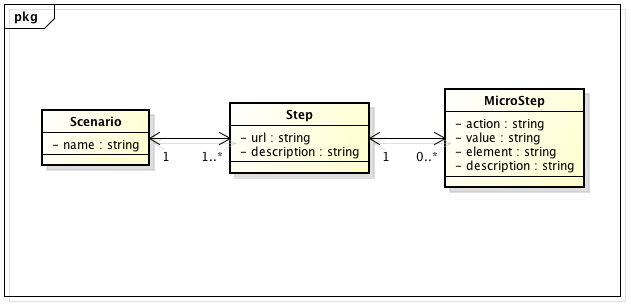
\includegraphics[width=0.9 \textwidth]{figuras/figura_32}
    \caption{Diagrama de classes da arquitetura inicial}
    \label{figura_32}
\end{figure}

Entretanto, após implementada esta arquitetura pode-se verificar a dificuldade na utilização da ferramenta. Foi então realizado um refatoramento que levou a descoberta de uma biblioteca da linguagem \textit{Ruby} (\textit{Hashr}) que facilitou uma nova arquitetura.

A biblioteca \textit{Hashr} cria uma nova classe derivada da classe \textit{Hash}, que simplifica o uso de \textit{hashes} aninhados e acesso aos seus valores \cite{HASHR}. O Código \ref{lst:codigo36} exemplifica o uso desta estrutura.

{\singlespace
\begin{lstlisting}[caption=Exemplo de uso da estrutura \textit{Hashr},label={lst:codigo36}]
monografia = Hashr.new titulo: 'Documentacao Executavel',
                       autores: {autor_1: 'Tiago', autor_2: 'Natanael'}

monografia.titulo  # => 'Documentacao Executavel'
monografia.autor_1 # => 'Tiago'
monografia.autor_2 # => 'Natanael'

\end{lstlisting}
}

Porém o exemplo acima não é a melhor representação da estrutura desejada. Os autores devem pertencer a uma lista, entretanto o \textit{Hashr} não converte os itens da lista conforme esperado. Para resolver este problema, foi desenvolvido um método recursivo que converte os valores em lista produzindo assim os efeitos esperados (Código \ref{lst:codigo37}).

{\singlespace
\begin{lstlisting}[caption=Método de conversão para \textit{Hashr},label={lst:codigo37}]
monografia = Hashr.new titulo: 'Documentacao Executavel',
                       autores: [{nome: 'Tiago'}, {nome: 'Natanael'}]

monografia.autores.first.nome # => NoMethodError

def convert_to_hashr(hash)
 hash = Hashr.new(hash)
 hash.values.find_all { |value| value.is_a?(Array) }.each do |value|
   value.each_index do |i|
     value[i] = convert_to_hashr(value[i]) if value[i].is_a? Hash
   end
 end
 hash
end

monografia = convert_to_hashr(monografia)
monografia.autores.first.nome  # => 'Tiago'
\end{lstlisting}
}

Com essa abordagem, foi possível criar uma estrutura simples de dicionários e listas para representar as classes \textit{Step} e \textit{MicroStep}, visto que essas classes eram pobres de lógica e serviam apenas para a estruturação e persistência de dados. Com essa estrutura foi possível fazer a simplificação da entrada de dados para o cadastro e gerenciamento dos cenários, usando o formato de serialização de dados \textit{YAML}.

A vantagem de utilizar este formato é que ele pode ser facilmente entendível por humanos e ao mesmo tempo é flexível e facilmente manipulável. Ele aceita representação para as estruturas de listas, dicionários e valores simples, como texto e inteiros \cite{YAML}. Usando esse formato de entrada, o cadastro de um novo cenário pode ser feita como exemplificado no Código \ref{lst:codigo38}.

{\singlespace
\begin{lstlisting}[caption=Exemplo de cenário escrito em \textit{YAML},label={lst:codigo38}]
scenario: Login de Usuario

contexts:
  - url: /
    steps:
      - description:
          Os links referentes ao acesso do usuario
          ficam no menu do canto superior direito
        element: actions
        padding: 3
        position: rmb

      - description: Clique na opcao 'Acesso'
        element: sign_in
        padding: 3
        position: rmb
        action: click

  - url: /usuarios/login
    steps:
      - description: Preencha o campo 'E-mail'
        element: usuario_email
        padding: 3
        position: tcc
        action: type
        value: exemplo@exemplo.com
      - description: Preencha o campo 'Senha'
        element: usuario_senha
        padding: 3
        position: tcc
        action: type
        value: exemplo123
      - description: Clique no botao 'Entrar'
        element: login
        padding: 3
        position: tcc
        action: click
\end{lstlisting}
}

 % Cria o capítulo 3
\chapter{CONSIDERAÇÕES FINAIS}

\section{Conclusões}

Com o trabalho realizado foi possível prototipar e avaliar uma ferramenta que possibilite ao usuário descrever os requisitos do sistema em forma de cenários. Essa conquista possibilitará a execução destes cenários em forma de tutorial guiado, trazendo um melhor entendimento do sistema, e tornando mais fácil e conexa a verificação de que todos os requisitos foram corretamente implementados.

O conceito que envolve a prototipação da ferramenta, levou a discussão da documentação tradicional e executável. Em um projeto tradicional, as constantes modifições dos requisitos do sistema geram problemas de sincronização dos documentos escritos em papel. Já a documentação executável pôde ser descrita em linguagem natural, da mesma forma que a tradicional, porém pôde ser executada, e trouxe a vantagem da possibilidade de validar os cenários documentados automaticamente.

Espera-se com este trabalho ter demonstrado que o conceito da ferramenta de documentação executável pode ser utilizado por outros projetos, no intuito de oferecer ao cliente uma documentação que agregue mais valor ao seu sistema. Com isso os usuários poderão ser mais facilmente treinados, e ajudarão na validação dos módulos do sistema.

\section{Limitações}

\section{Trabalhos Futuros} % Cria o capítulo 4
\bibliography{referencias} % Gera as referências bibliográficas
\end{document} % Fim do TCC
